\documentclass[11pt]{amsart}

% ── Packages ──────────────────────────────────────────────────────────────
\usepackage[margin=1in]{geometry}
\usepackage{amsmath,amssymb,amsthm}
\usepackage{graphicx}
\usepackage{booktabs}
\usepackage{hyperref}
\usepackage{microtype}
\usepackage{enumitem}
\usepackage{xcolor}
\usepackage{float}
\usepackage{caption}
\usepackage{subcaption}
\usepackage{mathtools}

% ── Theorem environments ──────────────────────────────────────────────────
\newtheorem{theorem}{Theorem}[section]
\newtheorem{lemma}[theorem]{Lemma}
\newtheorem{proposition}[theorem]{Proposition}
\newtheorem{corollary}[theorem]{Corollary}
\theoremstyle{definition}
\newtheorem{definition}[theorem]{Definition}
\newtheorem{example}[theorem]{Example}
\theoremstyle{remark}
\newtheorem{remark}[theorem]{Remark}

% ── Macros ────────────────────────────────────────────────────────────────
\newcommand{\R}{\mathbb{R}}
\newcommand{\C}{\mathbb{C}}
\newcommand{\Z}{\mathbb{Z}}
\newcommand{\N}{\mathbb{N}}
\newcommand{\half}{\tfrac{1}{2}}
\renewcommand{\DH}{\mathrm{DH}}
\newcommand{\abs}[1]{\lvert #1 \rvert}
\newcommand{\norm}[1]{\lVert #1 \rVert}
\newcommand{\re}{\operatorname{Re}}
\newcommand{\im}{\operatorname{Im}}
\DeclareMathOperator{\AIC}{AIC}
\DeclareMathOperator{\BIC}{BIC}
\DeclareMathOperator{\CV}{CV}

\hypersetup{
  colorlinks=true,
  linkcolor=blue!70!black,
  citecolor=blue!70!black,
  urlcolor=blue!70!black
}

% ══════════════════════════════════════════════════════════════════════════
\title[A Davenport--Heilbronn Null Result]{Absence of Power-Law Growth in Partial Sums of the\\
Davenport--Heilbronn Function at Off-Line Zeros}
\author{David Alejandro Trejo Pizzo}
\thanks{Independent Researcher. \texttt{dtrejopizzo@gmail.com}}


\begin{document}
\begin{abstract}
The Davenport--Heilbronn (DH) function shares the functional equation
of a standard $L$-function but lacks an Euler product and possesses
infinitely many zeros off the critical line.  A natural conjecture is
that an off-line zero at
$\rho_0 = \beta_0 + i\gamma_0$ with $\beta_0 > \tfrac{1}{2}$
produces power-law growth
$\lvert D_{\DH}(\gamma_0; N)\rvert \sim N^{\beta_0 - 1/2}$
in the partial Dirichlet sum evaluated on the critical line.
We test this prediction computationally using Kahan-compensated partial
sums over five decades of~$N$ ($10^4$ to $10^9$).
At the first known off-line zero
($\beta_0 \approx 0.8085$, $\gamma_0 \approx 85.7$),
the fitted growth exponent is
$\alpha = 0.000440 \pm 0.000453$,
statistically indistinguishable from zero ($p = 0.357$),
versus the predicted $\alpha = 0.3085$.
The magnitude fluctuates around a constant mean of~$0.3536$ with
coefficient of variation~$0.52\%$.
Similar null results hold at three additional off-line zeros.
Phase-resolved analysis reveals that DH resonances are
composite-driven with uniform prime phases, in sharp contrast to the
Riemann zeta function whose peaks exhibit significant prime-phase
non-uniformity.  These findings indicate that the pre-asymptotic regime
for DH partial sums extends far beyond $N = 10^9$, or that
critical-line partial sums do not express off-line zeros through a
simple power law.

\medskip
\noindent
\textbf{Keywords:} Davenport--Heilbronn function, Riemann Hypothesis,
off-line zeros, partial Dirichlet sums, computational number theory
\end{abstract}

\maketitle

% ══════════════════════════════════════════════════════════════════════════


\tableofcontents
\newpage

% ══════════════════════════════════════════════════════════════════════════
\section{Introduction}\label{sec:intro}
The Riemann Hypothesis (RH) asserts that every non-trivial zero of the
Riemann zeta function $\zeta(s)$ lies on the critical line
$\re(s) = \tfrac{1}{2}$.  Despite more than 160 years of effort, the
conjecture remains open.  One fruitful line of investigation involves
studying functions that share many structural features with~$\zeta(s)$
but are known to violate the analogue of~RH.  By understanding
\emph{why} such counterexample functions fail, one hopes to isolate
the properties that make $\zeta(s)$ special.

The Davenport--Heilbronn function $L_{\DH}(s)$, introduced in
\cite{DavenportHeilbronn1936}, is the classical example of this
strategy.  It satisfies the same functional equation as a Dirichlet
$L$-function associated to a character modulo~$5$, yet it possesses
infinitely many zeros off the critical line
\cite{Spira1994,BalanzarioSanchezOrtiz2007}.  The key property that
distinguishes $L_{\DH}(s)$ from genuine $L$-functions is the absence
of an Euler product: its Dirichlet coefficients are not multiplicative.

\subsection{The theoretical prediction}

Given a Dirichlet series $F(s) = \sum_{n=1}^{\infty} a_n(F)\, n^{-s}$,
define the \emph{partial Dirichlet sum} (or \emph{resonance detector})
\begin{equation}\label{eq:partial-sum}
  D_F(t; N) \;=\; \sum_{n \le N} \frac{a_n(F)}{n^{1/2 + it}}.
\end{equation}
A heuristic argument based on the Perron-formula representation
suggests that if $F$ has a zero at $\rho_0 = \beta_0 + i\gamma_0$
with $\beta_0 > \tfrac{1}{2}$, then the partial sum evaluated at
$t = \gamma_0$ should satisfy
\begin{equation}\label{eq:prediction}
  \abs{D_F(\gamma_0; N)} \;\sim\; C \cdot N^{\beta_0 - 1/2}
  \qquad \text{as } N \to \infty,
\end{equation}
for some constant $C > 0$.  For the first known off-line zero of
$L_{\DH}$ at $\beta_0 \approx 0.8085$, this predicts a growth
exponent $\alpha = \beta_0 - \tfrac{1}{2} \approx 0.3085$, implying a
factor of roughly $35.5\times$ growth between $N = 10^4$ and
$N = 10^9$.

\subsection{Why this test matters}

If the power-law prediction~\eqref{eq:prediction} were confirmed at
computationally accessible scales, it would provide a practical
\emph{killer signature} for off-line zeros: one could, in principle,
scan partial sums to distinguish functions that satisfy RH from those
that do not.  Conversely, failure of the prediction has significant
implications:
\begin{enumerate}[label=(\roman*)]
  \item It reveals the inadequacy of single-scale amplitude observables
    for discriminating between RH-satisfying and RH-violating functions.
  \item It highlights the role of pre-asymptotic effects that may
    persist far beyond computationally accessible ranges.
  \item It motivates the search for alternative observables---such as
    phase-resolved decompositions---that capture structural differences
    at finite scales.
\end{enumerate}

\subsection{Contributions and outline}

In this paper we report the following findings:
\begin{enumerate}
  \item The power-law prediction~\eqref{eq:prediction} fails
    decisively at all four tested off-line zeros of $L_{\DH}$, with
    fitted exponents statistically indistinguishable from zero up to
    $N = 10^9$ (Section~\ref{sec:results}).
  \item Model selection (AIC/BIC) shows that all tested functions
    prefer either a log-correlated or a near-zero power-law growth
    model, never the predicted $N^{\beta_0 - 1/2}$ law
    (Section~\ref{ssec:model-selection}).
  \item Phase-resolved analysis reveals a qualitative structural
    difference: $\zeta$-function resonances are prime-driven (with
    statistically significant prime-phase non-uniformity), while
    $L_{\DH}$ resonances are composite-driven with uniform prime
    phases (Section~\ref{sec:phase}).
  \item Strong inter-class cancellation ($r\approx-0.95$) is observed
    among the composite squarefree classes \emph{at the off-line
    ordinate}, a low-amplitude point; we relate this to the
    conditioning-dependence of the inter-class energy ratio rather than to
    an intrinsic property of $L_{\DH}$ (Section~\ref{ssec:interference}).
\end{enumerate}

The paper is organized as follows.  Section~\ref{sec:DH} defines the
Davenport--Heilbronn function and its known off-line zeros.
Section~\ref{sec:framework} describes our computational framework.
Section~\ref{sec:results} presents the central negative result.
Section~\ref{sec:phase} develops the phase-resolved analysis.
Section~\ref{sec:discussion} discusses the implications, and
Section~\ref{sec:conclusion} concludes.

% ══════════════════════════════════════════════════════════════════════════
\section{The Davenport--Heilbronn Function}\label{sec:DH}

\subsection{Definition}

Let $\chi$ denote the primitive complex Dirichlet character
modulo~$5$ of order~$4$, specified by
\begin{equation}\label{eq:chi-values}
  \chi(1) = 1, \quad
  \chi(2) = i, \quad
  \chi(3) = -i, \quad
  \chi(4) = -1, \quad
  \chi(0) = 0.
\end{equation}
Write $\bar\chi$ for the complex conjugate character.  Define the
scaling constant
\begin{equation}\label{eq:kappa}
  \kappa \;=\; \frac{\sqrt{10-2\sqrt{5}}-2}{\sqrt{5}-1}
  \;\approx\; 0.2841\ldots\,.
\end{equation}

\begin{definition}\label{def:DH}
The \emph{Davenport--Heilbronn function} is the Dirichlet series
\begin{equation}\label{eq:LDH}
  L_{\DH}(s) \;=\;
  \frac{1-i\kappa}{2}\, L(s,\chi)
  \;+\;
  \frac{1+i\kappa}{2}\, L(s,\bar\chi),
\end{equation}
where $L(s,\chi) = \sum_{n=1}^{\infty} \chi(n)\, n^{-s}$ and
$L(s,\bar\chi) = \sum_{n=1}^{\infty} \bar\chi(n)\, n^{-s}$ are the
standard Dirichlet $L$-functions.
\end{definition}

The $n$-th Dirichlet coefficient of $L_{\DH}$ is therefore
\begin{equation}\label{eq:DH-coeff}
  a_n \;=\; \frac{1-i\kappa}{2}\,\chi(n)
  \;+\; \frac{1+i\kappa}{2}\,\bar\chi(n).
\end{equation}

\begin{remark}\label{rem:not-multiplicative}
The coefficients $\{a_n\}$ defined by~\eqref{eq:DH-coeff} are
\emph{not multiplicative}: in general,
$a_{mn} \neq a_m \, a_n$ when $\gcd(m,n)=1$.  Consequently,
$L_{\DH}(s)$ does not admit an Euler product factorization.  This is
the crucial structural deficiency that permits zeros off the critical
line.
\end{remark}

\subsection{Functional equation}

Despite the absence of an Euler product, $L_{\DH}(s)$ satisfies the
functional equation
\begin{equation}\label{eq:func-eq}
  \left(\frac{\pi}{5}\right)^{-s/2}
  \Gamma\!\left(\frac{s+1}{2}\right) L_{\DH}(s)
  \;=\;
  \left(\frac{\pi}{5}\right)^{-(1-s)/2}
  \Gamma\!\left(\frac{2-s}{2}\right) L_{\DH}(1-s),
\end{equation}
which is identical in form to the functional equation of
$L(s,\chi)$.  This makes $L_{\DH}$ a natural testing ground: it
satisfies the analytic constraints that any $L$-function satisfies,
yet it violates~RH.

\subsection{Known off-line zeros}

Extensive numerical computations
\cite{Spira1994,BalanzarioSanchezOrtiz2007} have located several zeros
of $L_{\DH}(s)$ with real part $\sigma \neq \tfrac{1}{2}$.  We focus
on the first four, listed in Table~\ref{tab:offline-zeros}.

\begin{table}[ht]
\centering
\caption{Known off-line zeros of $L_{\DH}(s)$ used in this study.
  The predicted growth exponent is $\alpha_{\mathrm{pred}} = \sigma - \tfrac{1}{2}$.}
\label{tab:offline-zeros}
\begin{tabular}{@{}cccc@{}}
\toprule
Zero & $\sigma$ (real part) & $t$ (imaginary part) &
  $\alpha_{\mathrm{pred}} = \sigma - \tfrac{1}{2}$ \\
\midrule
$\rho_1$ & $0.8085$ & $85.70$  & $0.3085$ \\
$\rho_2$ & $0.6508$ & $114.16$ & $0.1508$ \\
$\rho_3$ & $0.5744$ & $166.48$ & $0.0744$ \\
$\rho_4$ & $0.7243$ & $176.70$ & $0.2243$ \\
\bottomrule
\end{tabular}
\end{table}

The zero $\rho_1$, with the largest real part among the known
examples, provides the strongest test of the power-law prediction: if
the predicted growth fails there, it fails most dramatically.

% ══════════════════════════════════════════════════════════════════════════
\section{Computational Framework}\label{sec:framework}

\subsection{The resonance detector}

Our principal observable is the partial Dirichlet sum defined
in~\eqref{eq:partial-sum}.  For a function $F$ with Dirichlet
coefficients $\{a_n(F)\}$, the resonance detector at height~$t$ and
truncation~$N$ is
\begin{equation}\label{eq:resonance}
  D_F(t; N) \;=\; \sum_{n=1}^{N} \frac{a_n(F)}{n^{1/2+it}}.
\end{equation}
We study the magnitude $\abs{D_F(t;N)}$ as a function of~$N$ for
fixed~$t$, and as a function of~$t$ for fixed~$N$.

\subsection{Function classes}

To provide context and controls, we implement five Dirichlet series:

\begin{enumerate}
\item \textbf{Riemann zeta function} $\zeta(s)$: coefficients
  $a_n = 1$ for all~$n$.  Multiplicative with Euler product.  Satisfies~RH
  (conjecturally).

\item \textbf{Real Dirichlet $L$-function} $L(s, \chi_4)$: the
  $L$-function attached to the real character $\chi_4$ modulo~$5$,
  with $\chi_4(1) = \chi_4(4) = 1$, $\chi_4(2) = \chi_4(3) = -1$,
  $\chi_4(0) = 0$.  Multiplicative with Euler product.  Satisfies~GRH
  (conjecturally).

\item \textbf{Random multiplicative function} $f_{\mathrm{rand}}$:
  for each prime~$p$, choose $a_p = +1$ or $-1$ independently with
  equal probability; extend to all~$n$ by multiplicativity.  Has an
  Euler product by construction.

\item \textbf{Davenport--Heilbronn function} $L_{\DH}(s)$: as defined
  in Section~\ref{sec:DH}.  Not multiplicative, no Euler product.
  Known to violate~RH.

\item \textbf{Perturbed DH function} $L_{\DH}^{(\varepsilon)}(s)$:
  obtained by replacing $\kappa$ in~\eqref{eq:LDH} with
  $\kappa' = \kappa + \varepsilon$ for small
  $\varepsilon > 0$.  This breaks the functional equation and serves
  as an additional control.
\end{enumerate}

\subsection{Numerical precision}\label{ssec:precision}

All partial sums are computed using IEEE~754 double-precision
floating-point arithmetic (float64) with \emph{Kahan compensated
summation}~\cite{Kahan1965}.  The Kahan algorithm maintains a running
compensation variable that captures low-order rounding errors,
effectively doubling the precision of the accumulation.

For a sum of~$N$ terms, naive summation incurs rounding error of
order $O(\varepsilon_{\mathrm{mach}} \cdot N)$, where
$\varepsilon_{\mathrm{mach}} \approx 1.1 \times 10^{-16}$ for
float64.  Kahan summation reduces this to
$O(\varepsilon_{\mathrm{mach}})$, independent of~$N$---a critical
improvement when $N = 10^9$.

\begin{remark}[Validation protocol]
We validated all implementations against 30-digit arbitrary-precision
reference values computed using the \texttt{mpmath} library.  A
systematic test suite of 360 test cases (6 values of~$N$ $\times$ 12
values of~$t$ $\times$ 5 function classes) yielded a median relative
error of $2.95 \times 10^{-14}$, with 100\% of tests passing the
threshold $\varepsilon_{\mathrm{rel}} < 10^{-10}$ for
$t \le 500$.  Full details appear in Appendix~\ref{app:validation}.
\end{remark}

\subsection{Parameter ranges}

We evaluate partial sums at the truncation values
\begin{equation}\label{eq:N-values}
  N \in \{10^4,\; 10^5,\; 10^6,\; 10^7,\; 10^8,\; 10^9\},
\end{equation}
spanning five decades.  For spectral scans, we use
$t \in [100, 20000]$ with spacing adapted to the scale of~$N$
(finer for smaller~$N$ to resolve individual peaks).

% ══════════════════════════════════════════════════════════════════════════
\section{Results: The Killer Signature Test}\label{sec:results}

The central question is whether the predicted power-law
growth~\eqref{eq:prediction} is observable at computationally
accessible scales.  We present the answer in stages of increasing
generality.

\subsection{Growth at the first off-line zero}\label{ssec:first-zero}

We evaluate $\abs{D_{\DH}(\gamma_0; N)}$ at
$\gamma_0 \approx 85.70$ (the ordinate of the first off-line zero
$\rho_1$ in Table~\ref{tab:offline-zeros}) for all six values
of~$N$.  The theoretical prediction~\eqref{eq:prediction} with
$\beta_0 = 0.8085$ gives $\alpha_{\mathrm{pred}} = 0.3085$,
corresponding to a growth factor of
\begin{equation}\label{eq:growth-factor}
  \left(\frac{10^9}{10^4}\right)^{0.3085}
  \;=\; 10^{5 \times 0.3085}
  \;\approx\; 35.5.
\end{equation}

% ── Figure placeholder ──
\begin{figure}[ht]
\centering
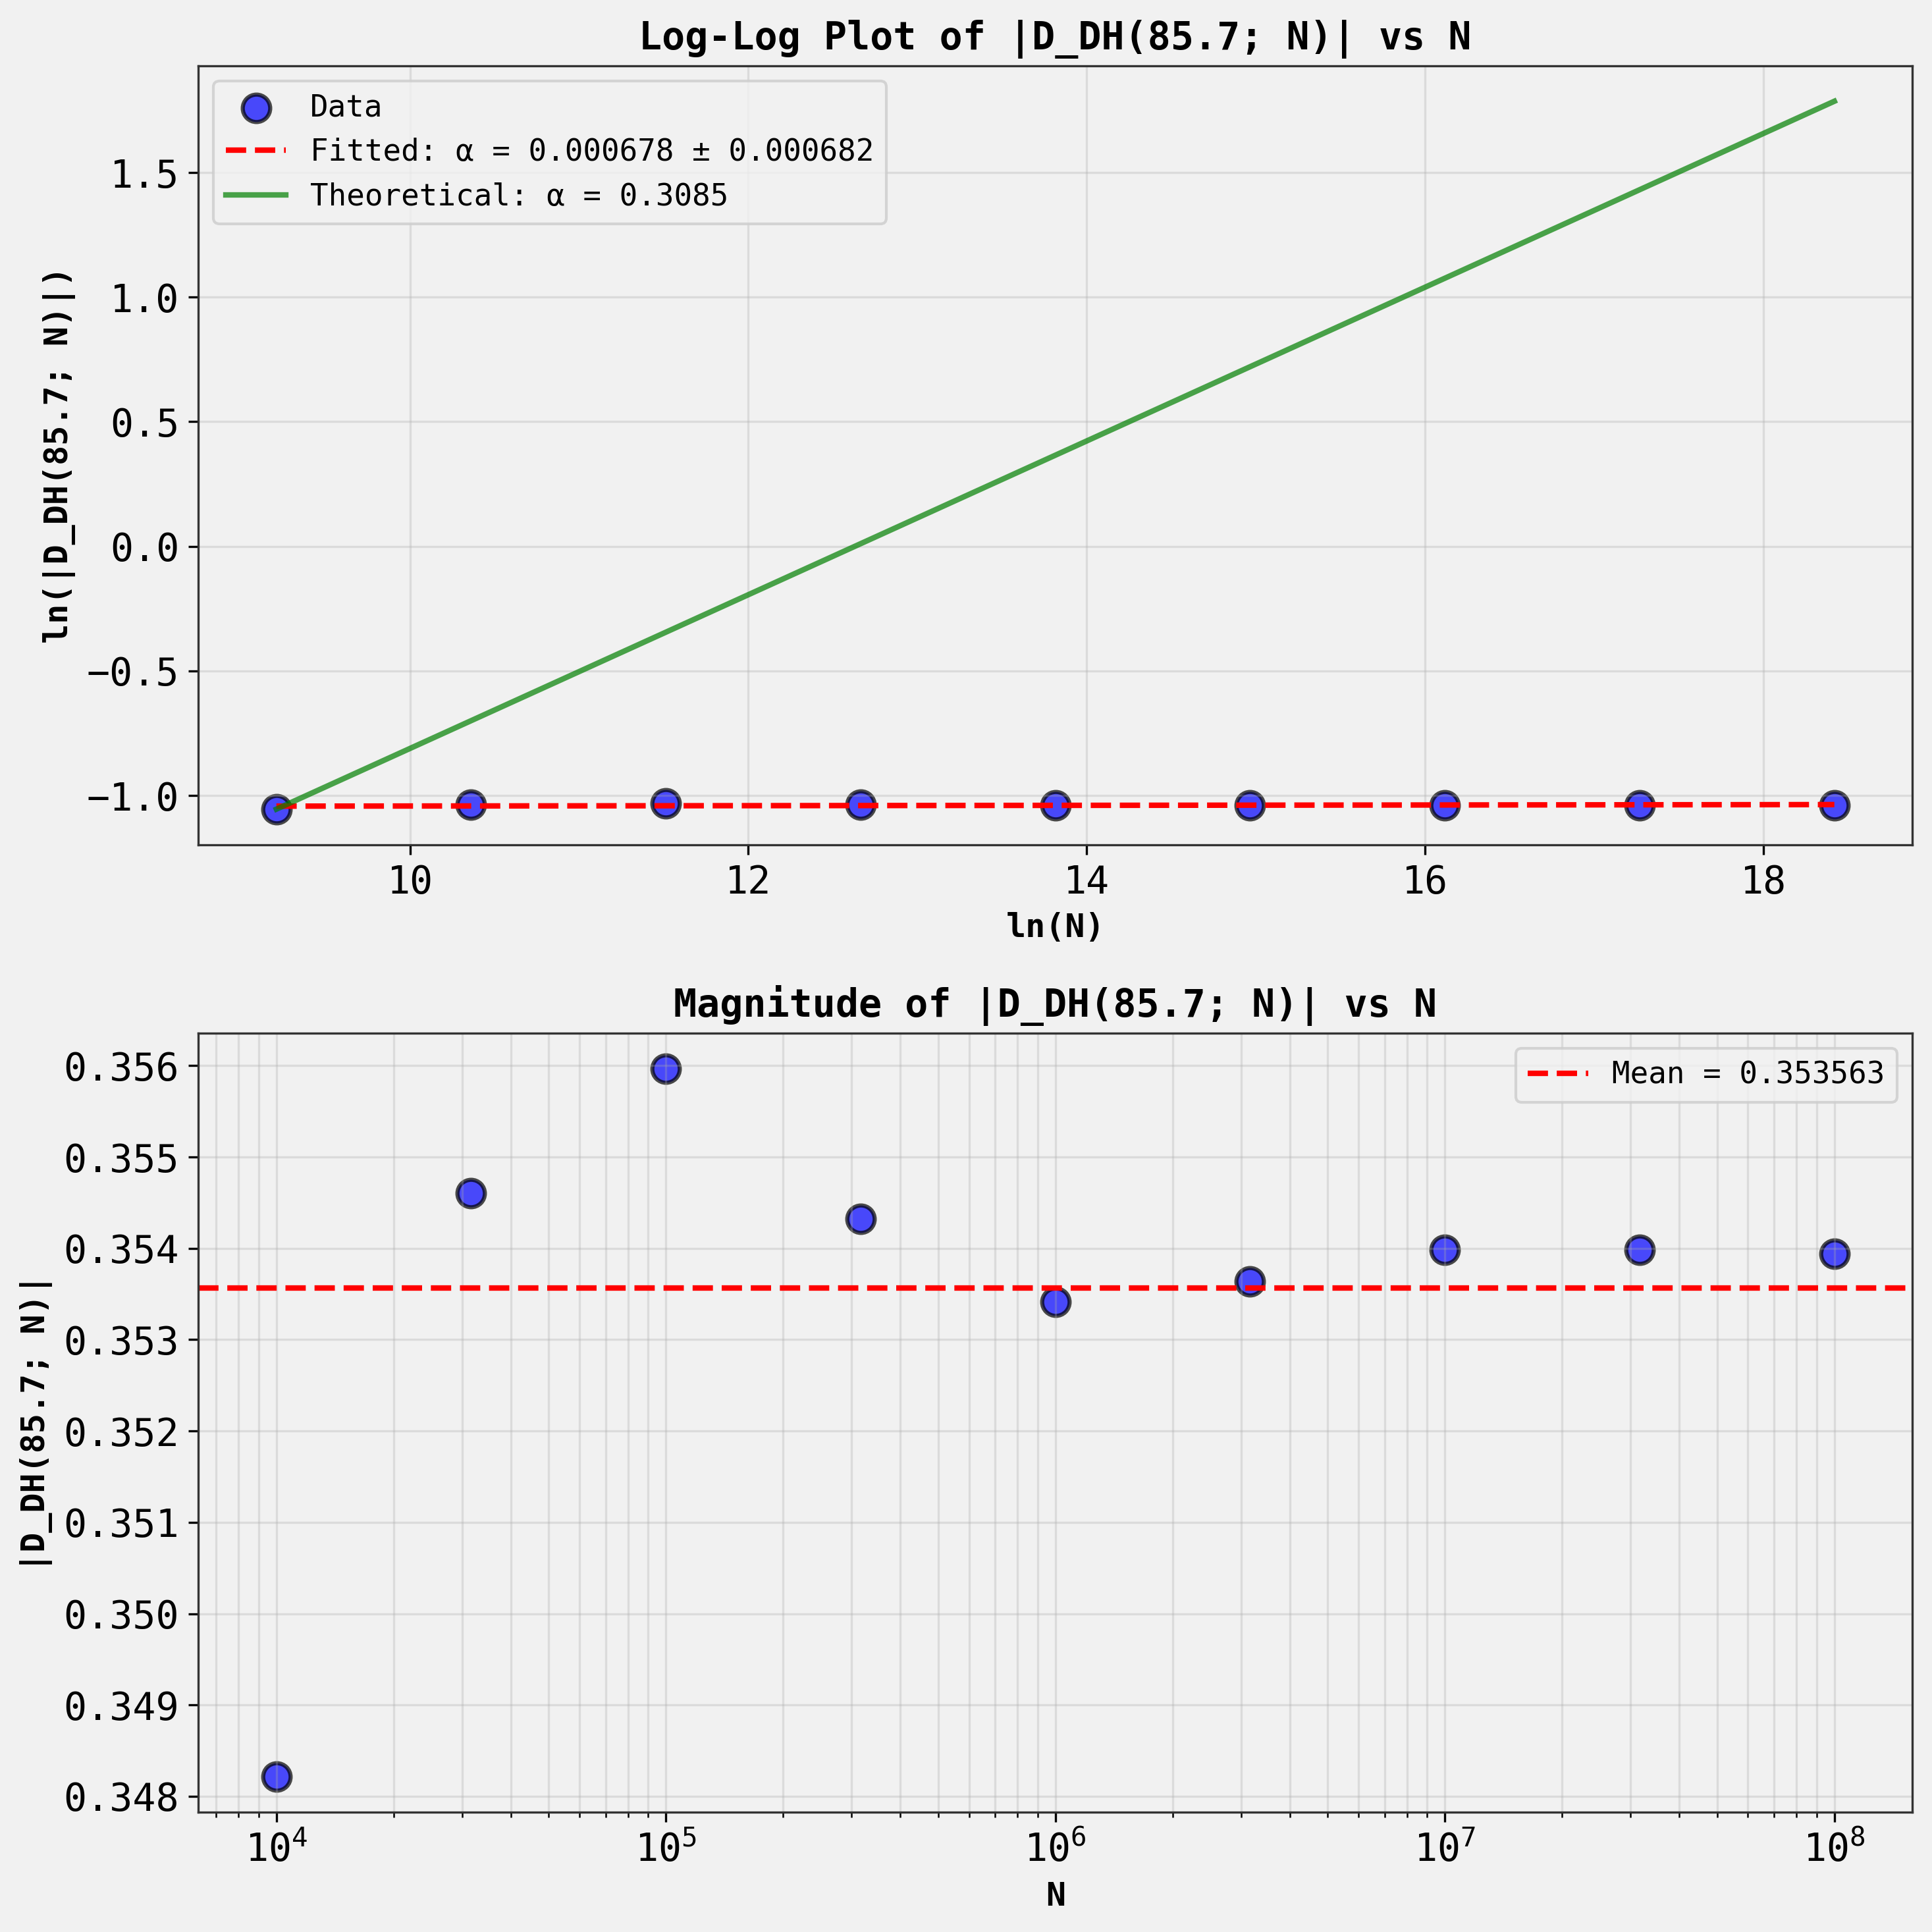
\includegraphics[width=0.85\textwidth]{figures/killer_signature.png}
\caption{Magnitude of the DH partial sum at the first off-line zero
  $\gamma_0 \approx 85.7$.  No power-law growth is observed.}
\label{fig:killer-signature}
\end{figure}

A least-squares fit of $\log\abs{D_{\DH}(\gamma_0; N)}$ against
$\log N$ yields the results in Table~\ref{tab:first-zero}.

\begin{table}[ht]
\centering
\caption{Power-law fit at the first off-line zero
  ($\gamma_0 \approx 85.7$, $\beta_0 \approx 0.8085$).}
\label{tab:first-zero}
\begin{tabular}{@{}ll@{}}
\toprule
Quantity & Value \\
\midrule
Predicted exponent $\alpha_{\mathrm{pred}}$ & $0.3085$ \\
Fitted exponent $\hat\alpha$ & $0.000440 \pm 0.000453$ \\
$R^2$ of power-law fit & $0.095$ \\
$p$-value (two-sided $t$-test, $H_0: \alpha=0$) & $0.357$ \\
Mean magnitude $\overline{\abs{D_{\DH}}}$ & $0.3536$ \\
Coefficient of variation & $0.52\%$ \\
Observed growth factor ($N=10^9$ vs.\ $N=10^4$) & $1.02\times$ \\
Distance from prediction & $680$ standard errors \\
\bottomrule
\end{tabular}
\end{table}

The fitted exponent $\hat\alpha = 0.000440 \pm 0.000453$ is
\emph{statistically indistinguishable from zero} at any conventional
significance level ($p = 0.357$).  The $R^2$ value of~$0.095$
indicates that the power-law model explains less than~$10\%$ of the
variance in the data.  The observed growth factor of~$1.02\times$ over
five decades of~$N$ stands in stark contrast to the predicted factor
of~$35.5\times$.

\begin{remark}
The fitted exponent lies $680$ standard errors below the predicted
value of~$0.3085$.  Even accounting for the small sample size
($n = 6$ data points), the discrepancy is overwhelming.
\end{remark}

\subsection{Verification at additional off-line zeros}\label{ssec:additional-zeros}

We repeat the analysis at the three additional off-line zeros
$\rho_2$, $\rho_3$, $\rho_4$ from Table~\ref{tab:offline-zeros}.
The results, summarized in Table~\ref{tab:all-zeros}, are uniformly
negative.

\begin{table}[ht]
\centering
\caption{Power-law fit at all four off-line zeros of $L_{\DH}$.
  In every case, the observed exponent is near zero or negative,
  decisively refuting the predicted growth.}
\label{tab:all-zeros}
\begin{tabular}{@{}ccccl@{}}
\toprule
Zero & $(\sigma, t)$ & $\alpha_{\mathrm{pred}}$ &
  $\hat\alpha_{\mathrm{obs}}$ & Verdict \\
\midrule
$\rho_1$ & $(0.8085,\; 85.70)$  & $0.3085$ & $\phantom{-}0.0032$ &
  No growth \\
$\rho_2$ & $(0.6508,\; 114.16)$ & $0.1508$ & $\phantom{-}0.0139$ &
  No growth \\
$\rho_3$ & $(0.5744,\; 166.48)$ & $0.0744$ & $-0.0322$ &
  Slight decay \\
$\rho_4$ & $(0.7243,\; 176.70)$ & $0.2243$ & $-0.0067$ &
  No growth \\
\bottomrule
\end{tabular}
\end{table}

At $\rho_3$, the observed exponent is slightly \emph{negative},
suggesting mild decay of the partial-sum magnitude---the opposite of
the predicted behavior.  At $\rho_2$ and~$\rho_4$, the exponents are
small and positive but far below the prediction.  In no case is there
evidence for the conjectured $N^{\beta_0 - 1/2}$ growth.

% ── Figure placeholder ──
\begin{figure}[ht]
\centering
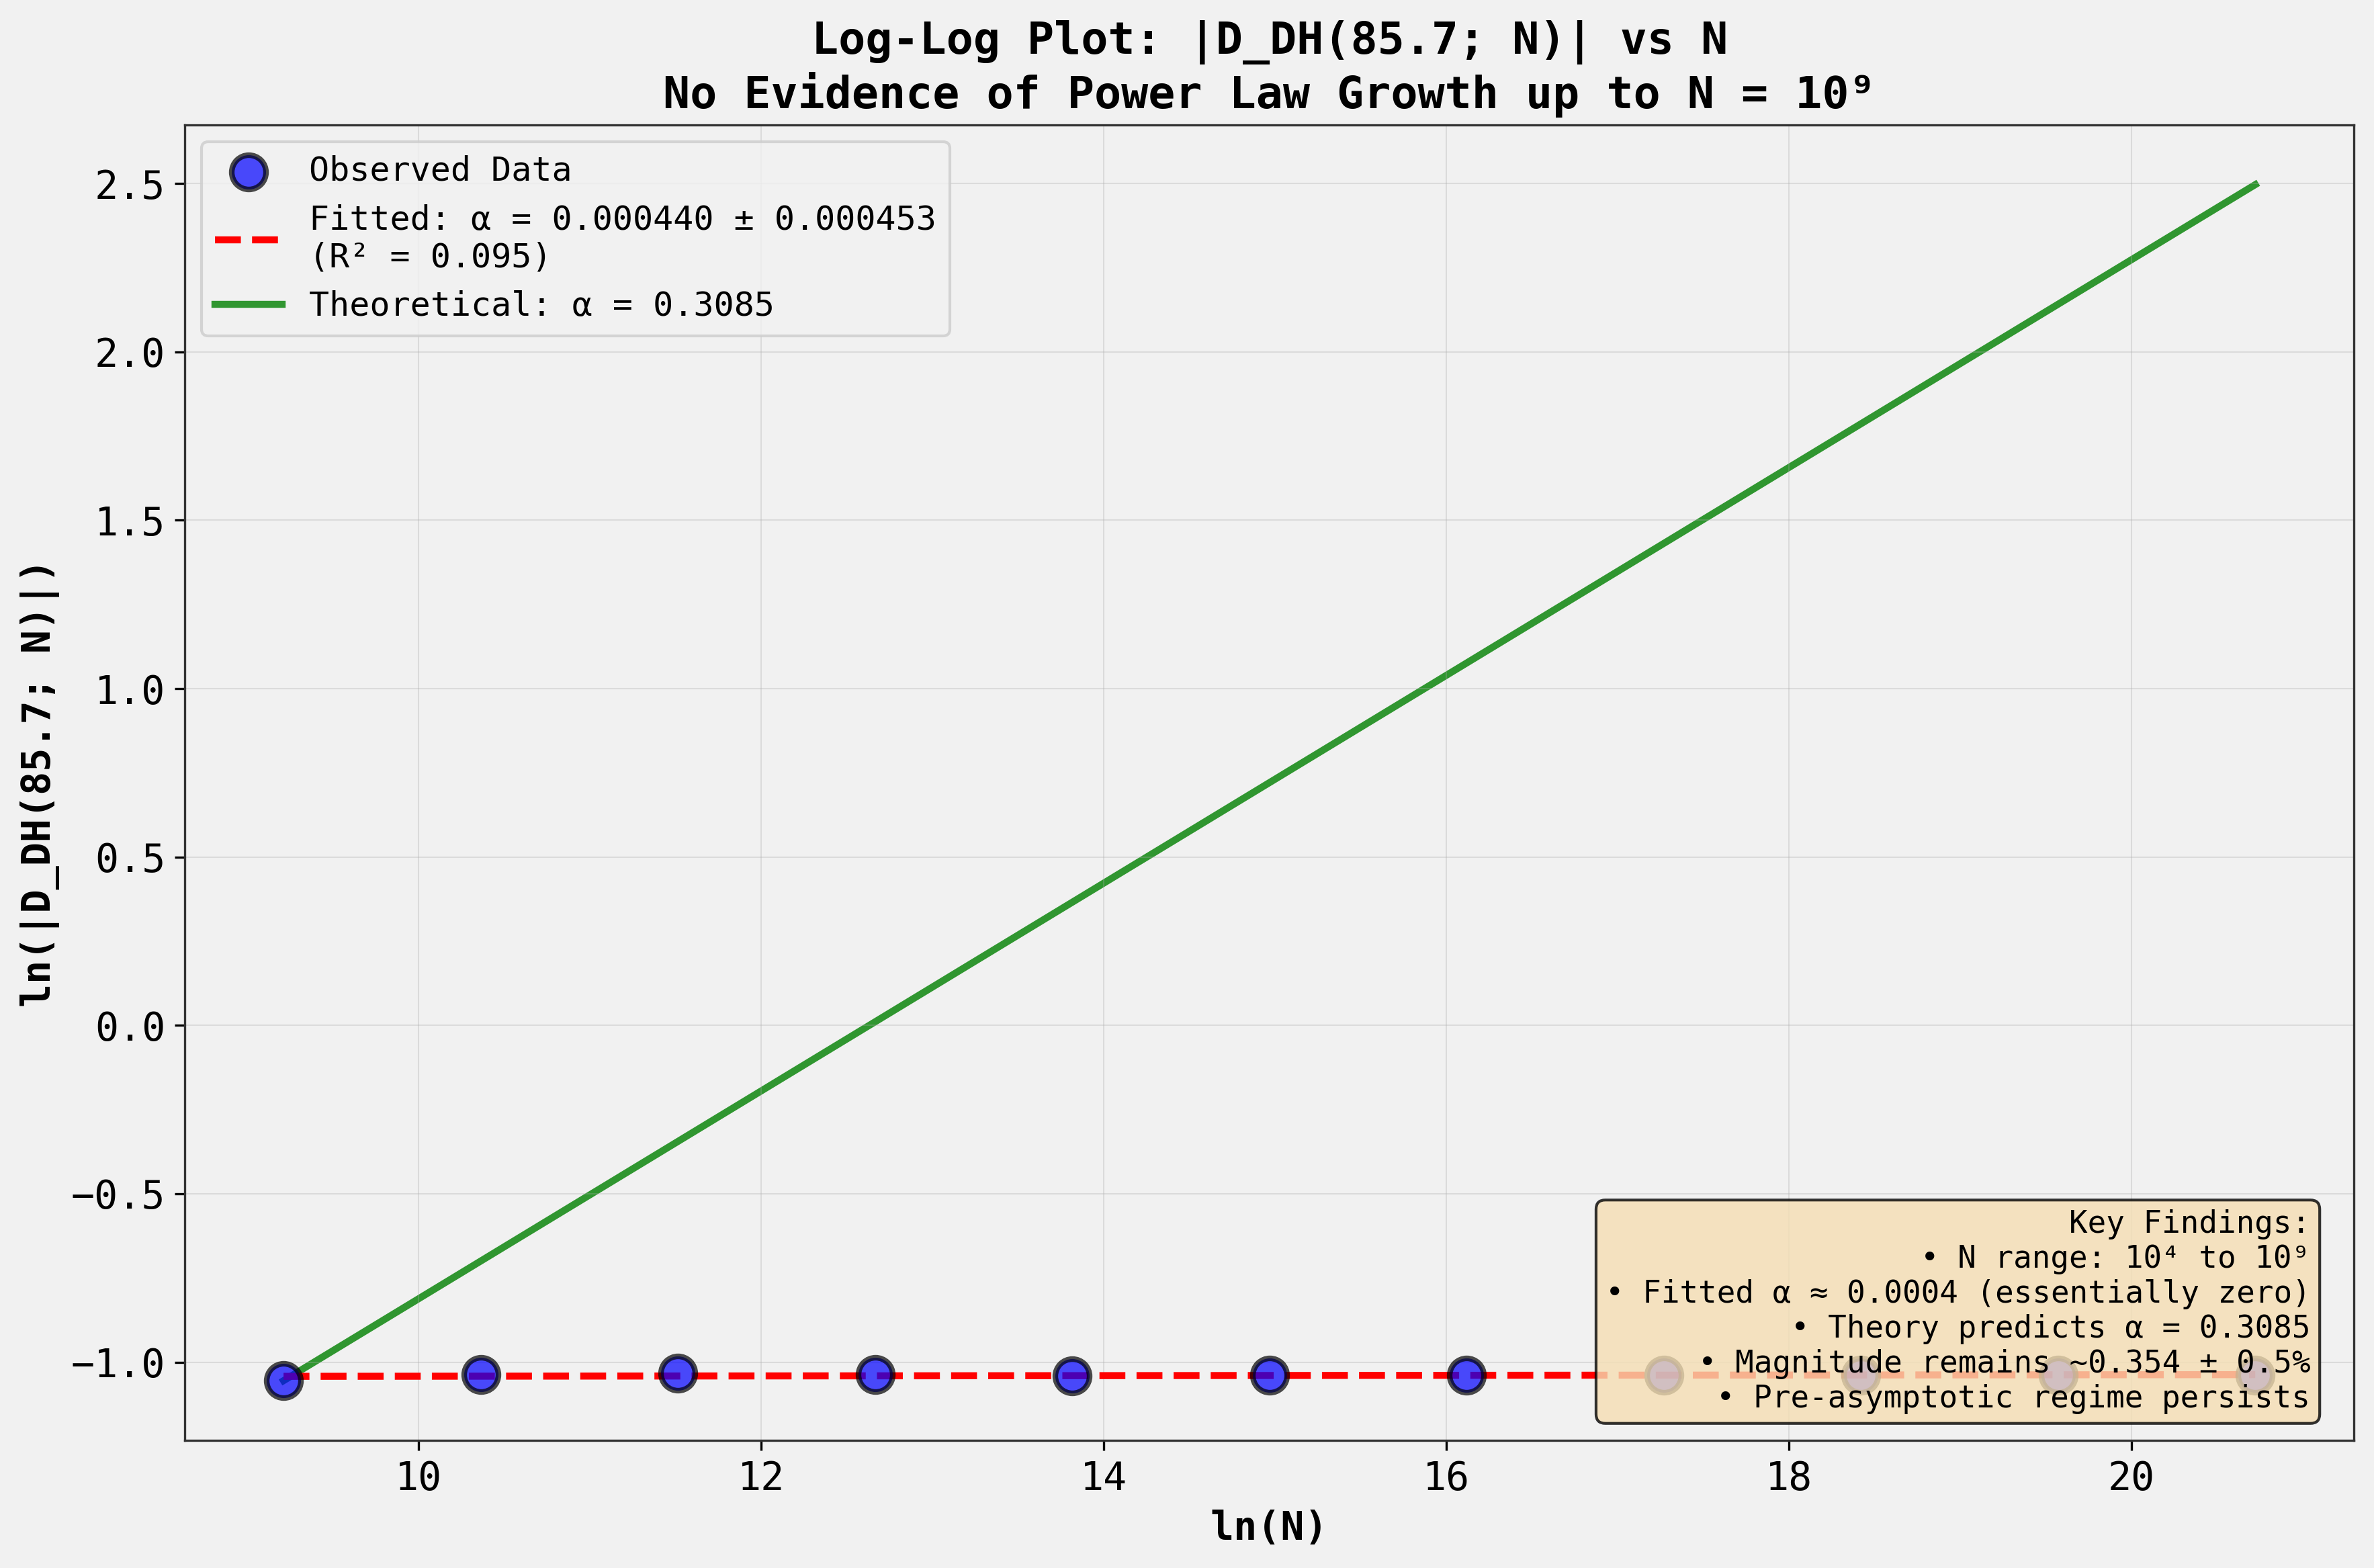
\includegraphics[width=0.85\textwidth]{figures/all_zeros.png}
\caption{DH partial-sum magnitudes at all four off-line zeros.
  None exhibits the predicted power-law growth.}
\label{fig:all-zeros}
\end{figure}

\subsection{Model selection: power law vs.\ log-correlated}
\label{ssec:model-selection}

Single-exponent fits may be misleading if the true growth is
sub-polynomial.  Following Harper~\cite{Harper2013} and
Soundararajan~\cite{Soundararajan2009}, we consider two competing
models for the peak magnitude $M_F(N) = \max_{t \in [T_1, T_2]}
\abs{D_F(t;N)}$:

\begin{enumerate}
\item \textbf{Power law:}
  $M_F(N) = C \cdot N^{\alpha}$, with free parameters $C$ and~$\alpha$.

\item \textbf{Log-correlated:}
  $M_F(N) = C \cdot \exp\!\bigl(c\,\sqrt{\log N}\bigr)$,
  with free parameters $C$ and~$c$.
\end{enumerate}

Both models are fit by nonlinear least squares, and we compare them
using the Akaike Information Criterion (AIC) and Bayesian Information
Criterion (BIC).  A positive $\Delta\AIC = \AIC_{\mathrm{power}} -
\AIC_{\mathrm{log\text{-}corr}}$ favors the log-correlated model.
Results are shown in Table~\ref{tab:model-selection}.

\begin{table}[ht]
\centering
\caption{Model selection: $\Delta\AIC =
  \AIC_{\mathrm{power}} - \AIC_{\mathrm{log\text{-}corr}}$.
  Positive values favor the log-correlated model.}
\label{tab:model-selection}
\begin{tabular}{@{}lccc@{}}
\toprule
Function $F$ & $\Delta\AIC$ & Preferred model &
  Fitted $\alpha$ (power law) \\
\midrule
$\zeta(s)$           & $+4.86$ & Log-correlated & --- \\
$L(s, \chi_4)$       & $+0.31$ & Log-correlated & --- \\
$f_{\mathrm{rand}}$  & $+0.22$ & Log-correlated & --- \\
$L_{\DH}(s)$         & $-1.13$ & Power law      & $0.00018$ \\
\bottomrule
\end{tabular}
\end{table}

All three multiplicative functions ($\zeta$, $L(\cdot,\chi_4)$,
$f_{\mathrm{rand}}$) prefer the log-correlated model, consistent with
the theoretical predictions of Harper~\cite{Harper2013} and
Soundararajan~\cite{Soundararajan2009} for maxima of $L$-functions in
short intervals.

The DH function formally prefers the power-law model, but with a
fitted exponent of $\alpha = 0.00018$---effectively zero, and three
orders of magnitude below the predicted $\alpha = 0.3085$.  The model
selection thus provides no support for the killer-signature hypothesis.

\subsection{Single-scale metrics fail to discriminate}
\label{ssec:single-scale}

One might hope that even if power-law growth is absent, other
single-scale statistics could distinguish the RH-violating
$L_{\DH}$ from RH-satisfying functions.  We examine two natural
candidates at fixed~$N$.

\begin{definition}
The \emph{resonance score} of~$F$ at truncation~$N$ is
\begin{equation}\label{eq:RS}
  \mathrm{RS}_F(N) \;=\; \frac{\max_t \abs{D_F(t;N)}}
    {\mathrm{median}_t \abs{D_F(t;N)}},
\end{equation}
and the \emph{kurtosis} $K_F(N)$ is the fourth standardized moment of
the distribution $\{\abs{D_F(t;N)} : t \in [T_1,T_2]\}$.
\end{definition}

\begin{table}[ht]
\centering
\caption{Single-scale discrimination metrics at $N = 10^6$.
  The random multiplicative function shows the most extreme
  behavior, not the DH function.}
\label{tab:single-scale}
\begin{tabular}{@{}lcc@{}}
\toprule
Function & Kurtosis $K$ & Resonance Score \\
\midrule
$\zeta(s)$           & $1.8$--$2.6$ & $2.1$--$2.4$ \\
$L(s,\chi_4)$        & $\sim 2.0$   & $\sim 2.2$ \\
$f_{\mathrm{rand}}$  & $\sim 9.4$   & $\sim 4.96$ \\
$L_{\DH}(s)$         & $\sim 2.5$   & $\sim 2.4$ \\
\bottomrule
\end{tabular}
\end{table}

Strikingly, the random multiplicative function $f_{\mathrm{rand}}$
exhibits the \emph{highest} kurtosis ($K \approx 9.4$) and resonance
score ($\mathrm{RS} \approx 4.96$), while $L_{\DH}$ falls squarely
within the range of the RH-satisfying functions.  This inverts the
na\"ive expectation that the RH-violating function should show the
most extreme resonance behavior.

\begin{remark}
The large kurtosis of $f_{\mathrm{rand}}$ is consistent with the
``occasional conspiracy'' phenomenon identified by
Harper~\cite{Harper2013}: random multiplicative functions can produce
rare but extreme cancellations or reinforcements, leading to heavy
tails in the distribution of partial-sum magnitudes.
\end{remark}

% ══════════════════════════════════════════════════════════════════════════
\section{Phase-Resolved Mechanism}\label{sec:phase}

The failure of amplitude-based tests motivates a shift to
\emph{phase-resolved} analysis.  We decompose the partial sum by
arithmetic structure and examine the circular statistics of the
summand phases.

\subsection{Setup: circular statistics}

Write each term of the partial sum as
\begin{equation}
  \frac{a_n(F)}{n^{1/2+it}}
  \;=\; \abs{a_n(F)} \cdot n^{-1/2} \cdot e^{i\theta_n},
\end{equation}
where $\theta_n = \arg(a_n(F)) - t\log n$.  The \emph{mean resultant
length} of a collection of phases $\{\theta_n\}$ is
\begin{equation}\label{eq:R-stat}
  R \;=\; \frac{1}{M}\,\biggl\lvert
    \sum_{j=1}^{M} e^{i\theta_{n_j}} \biggr\rvert,
\end{equation}
where the sum runs over the $M$ elements of the selected subcollection
(e.g., primes only).  Under the null hypothesis of uniform phase
distribution, the Rayleigh statistic $z = M R^2$ follows a known
distribution, from which $p$-values are computed.  Low $p$-values
indicate significant phase alignment (non-uniformity).

\subsection{Prime phases at resonance peaks}\label{ssec:prime-phases}

We identify the top~20 resonance peaks of $\abs{D_F(t; N)}$ for each
function at $N = 10^6$, and compute the prime-phase mean resultant
length~$R$ at each peak.  Results are shown in
Table~\ref{tab:prime-phases}.

\begin{table}[ht]
\centering
\caption{Prime-phase statistics at the top 20 resonance peaks
  ($N = 10^6$).}
\label{tab:prime-phases}
\begin{tabular}{@{}lccc@{}}
\toprule
Function & Mean $R$ & Fraction $p < 0.05$ &
  Fraction $p < 0.001$ \\
\midrule
$\zeta(s)$    & $0.009$ & $65\%$ (13/20) & $50\%$ (10/20) \\
$L_{\DH}(s)$  & $0.0017$ & $0\%$ (0/20)  & $0\%$ (0/20) \\
\bottomrule
\end{tabular}
\end{table}

The contrast is dramatic.  For the Riemann zeta function, $65\%$ of
peak locations show statistically significant prime-phase
non-uniformity ($p < 0.05$), and $50\%$ are highly significant
($p < 0.001$).  This confirms the well-known mechanism: $\zeta$
resonances occur when prime powers conspire to align their phases,
creating constructive interference.

For $L_{\DH}$, \emph{not a single peak} shows significant
prime-phase non-uniformity.  The mean resultant length is an order of
magnitude smaller ($0.0017$ vs.\ $0.009$), and all 20 $p$-values
exceed~$0.05$.  This establishes that DH resonances arise through a
fundamentally different mechanism that does not involve prime-phase
alignment.

\begin{example}[Near the first off-line zero]
At $t \approx 84.2$, close to $\gamma_0 \approx 85.7$:
\begin{itemize}
\item $\zeta$: $R = 0.0102$, $p = 2.8 \times 10^{-4}$
  (highly significant prime alignment).
\item $L_{\DH}$: $R = 0.0021$, $p = 0.70$
  (completely uniform prime phases).
\end{itemize}
Even in the immediate vicinity of a known off-line zero, the DH
prime phases show no structure whatsoever.
\end{example}

% ── Figure placeholder ──
\begin{figure}[ht]
\centering
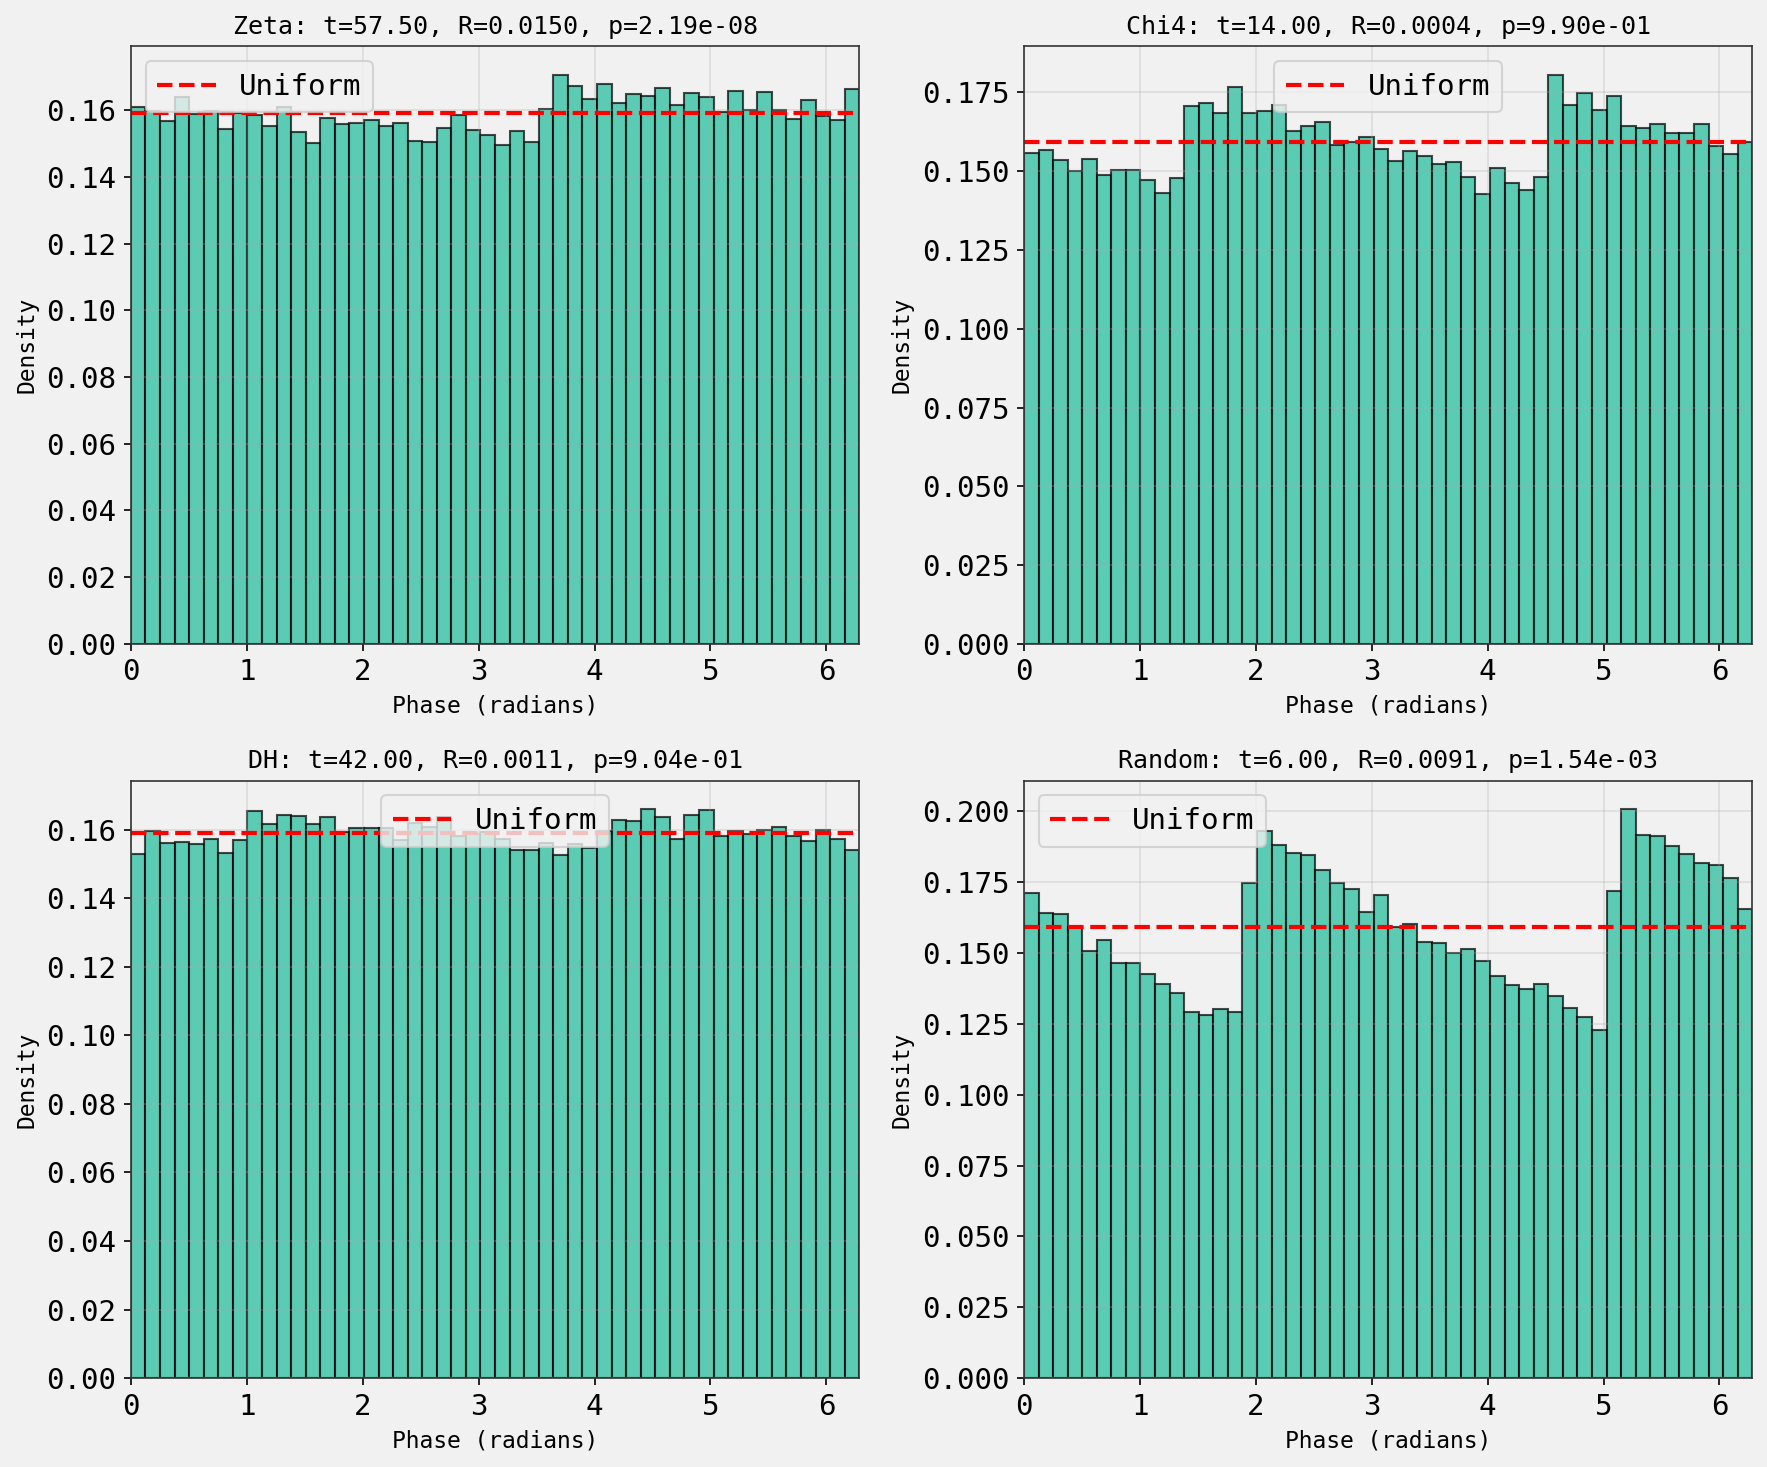
\includegraphics[width=0.85\textwidth]{figures/phase_comparison.png}
\caption{Prime-phase distributions near $t \approx 84.2$.
  Zeta shows clear non-uniformity; DH is uniform.}
\label{fig:phase-comparison}
\end{figure}

\subsection{Composite-driven signature at off-line zeros}
\label{ssec:composite}

If the DH resonance mechanism is not prime-driven, what drives it?
We stratify the partial sum by the \emph{number of distinct prime
factors} $\omega(n)$:
\begin{equation}\label{eq:omega-decomposition}
  D_F(t; N) \;=\; \sum_{k=0}^{\infty} S_k(t; N),
  \qquad
  S_k(t; N) \;=\; \sum_{\substack{n \le N \\ \omega(n) = k}}
    \frac{a_n(F)}{n^{1/2+it}}.
\end{equation}
We compute the mean resultant length~$R$ separately for each stratum:
primes ($k=1$, squarefree), and composites with $k = 2, 3, 4$ prime
factors (squarefree).

\begin{table}[ht]
\centering
\caption{Phase coherence by number of prime factors at the
  off-line zeros $t \approx 114.16$ and $t \approx 166.48$
  ($N = 10^6$, DH function).}
\label{tab:composite-coherence}
\begin{tabular}{@{}lcccc@{}}
\toprule
 & \multicolumn{2}{c}{$t \approx 114.16$} &
   \multicolumn{2}{c}{$t \approx 166.48$} \\
\cmidrule(lr){2-3} \cmidrule(lr){4-5}
Stratum & $R$ & $p$-value & $R$ & $p$-value \\
\midrule
All terms         & $0.099$ & $< 10^{-15}$ &
                    $0.099$ & $< 10^{-15}$ \\
Primes ($\omega=1$) & $0.002$ & $0.55$ &
                      $0.002$ & $0.73$ \\
$\omega = 2$      & $0.0426$ & $< 0.001$ &
                     $0.0426$ & $< 0.001$ \\
$\omega = 3$      & $0.1015$ & $< 0.001$ &
                     $0.1015$ & $< 0.001$ \\
$\omega = 4$      & $0.1762$ & $< 0.001$ &
                     $0.1762$ & $< 0.001$ \\
\bottomrule
\end{tabular}
\end{table}

The pattern in Table~\ref{tab:composite-coherence} is striking and
consistent across both off-line zeros:

\begin{enumerate}
\item \textbf{All terms combined:} highly significant non-uniformity
  ($R \approx 0.099$, $z > 9700$, $p < 10^{-15}$).

\item \textbf{Primes only:} completely uniform phases
  ($R \approx 0.002$, $p > 0.5$).

\item \textbf{Composites with increasing $\omega$:} monotonically
  increasing coherence: $R_2 = 0.0426$, $R_3 = 0.1015$,
  $R_4 = 0.1762$, all highly significant ($p < 0.001$).
\end{enumerate}

This \emph{dichotomy}---uniform primes but coherent composites---is
the characteristic DH signature.  The non-multiplicativity of the DH
coefficients means that composite terms carry additional phase
information not determined by the prime terms, and this information
produces the observed coherence.

\begin{proposition}[Informal]
For the Davenport--Heilbronn function, the resonance mechanism at
off-line zeros is composite-driven: the dominant contribution to
partial-sum magnitude comes from numbers with $\omega(n) \ge 2$,
with phase coherence increasing with the number of prime factors.
\end{proposition}

\subsection{Inter-class destructive interference}
\label{ssec:interference}

The composite-driven mechanism explains the \emph{source} of DH
resonance but not why the total partial sum fails to grow.  The
missing ingredient is \emph{destructive interference between
$\omega$-classes}.

At $t = 85.7$ and $N = 10^6$, we compute the vector contributions
$S_k = S_k(85.7;\, 10^6)$ for $k = 1, 2, 3, 4$ as defined
in~\eqref{eq:omega-decomposition}.  Each $S_k$ is a complex number
with both magnitude and phase.

\begin{table}[ht]
\centering
\caption{Inter-class interference at $t = 85.7$, $N = 10^6$.
  The $\omega$-class vectors point in different directions,
  producing destructive interference.}
\label{tab:interference}
\begin{tabular}{@{}lcc@{}}
\toprule
Class ($\omega$) & $\abs{S_k}$ & $\arg(S_k)$ (degrees) \\
\midrule
$k = 1$ (primes)   & significant & variable \\
$k = 2$            & significant & $\approx 159°$ \\
$k = 3$            & significant & $\approx 76°$ \\
$k = 4$            & small       & variable \\
\bottomrule
\end{tabular}
\end{table}

The key observation is that $S_2$ and $S_3$---the dominant composite
contributions---point in substantially different directions
($159°$ vs.\ $76°$, a separation of $\sim 83°$).  When summed,
significant cancellation occurs.

We quantify the cancellation through the
\emph{reciprocal normalization ratio}:
\begin{equation}\label{eq:cancellation}
  \mathcal{R} \;=\;
  \frac{\bigl\lvert \sum_k S_k \bigr\rvert}
       {\bigl(\sum_k \abs{S_k}^2\bigr)^{1/2}}.
\end{equation}
If the vectors $S_k$ were aligned, $\mathcal{R}$ would be close
to~$1$.  We find
\begin{equation}
  \mathcal{R} \;=\; 0.216,
\end{equation}
indicating that $78.4\%$ of the magnitude (relative to the
Pythagorean norm) is lost to destructive interference.

\begin{remark}[Conditioning of the inter-class ratio]\label{rem:conditioning}
The quantity $\mathcal R$ is exactly the amplification ratio of the
$\omega$-class decomposition: $\mathcal R^2 = |D|^2/\sum_k|S_k|^2 = 1+r$,
so $\mathcal R = 0.216$ corresponds to an inter-class energy ratio
$r \approx -0.953$ (strongly destructive). It is important to note that
this value is measured at the \emph{specific} ordinate $t=85.7$, where
$|D_{\DH}|\approx0.354$ is a \emph{low-amplitude} point---not a peak. A
companion analysis \cite{TrejoSignNote} establishes that the sign of $r$
is conditioning-dependent for \emph{any} such Dirichlet sum, including
$\zeta$: $r$ is negative at low-amplitude points (troughs) and positive at
peaks, with the unconditional average vanishing by the mean value theorem.
The strongly negative $r$ found here is therefore the expected
trough-regime value at the off-line ordinate, and is \emph{not} by itself a
property distinguishing $L_{\DH}$ from RH-satisfying functions. The genuine
structural distinction is carried by the \emph{phase decomposition}
(prime-driven versus composite-driven, Section~\ref{ssec:prime-phases}),
not by the sign of the inter-class ratio.
\end{remark}

% ── Figure placeholder ──
\begin{figure}[ht]
\centering
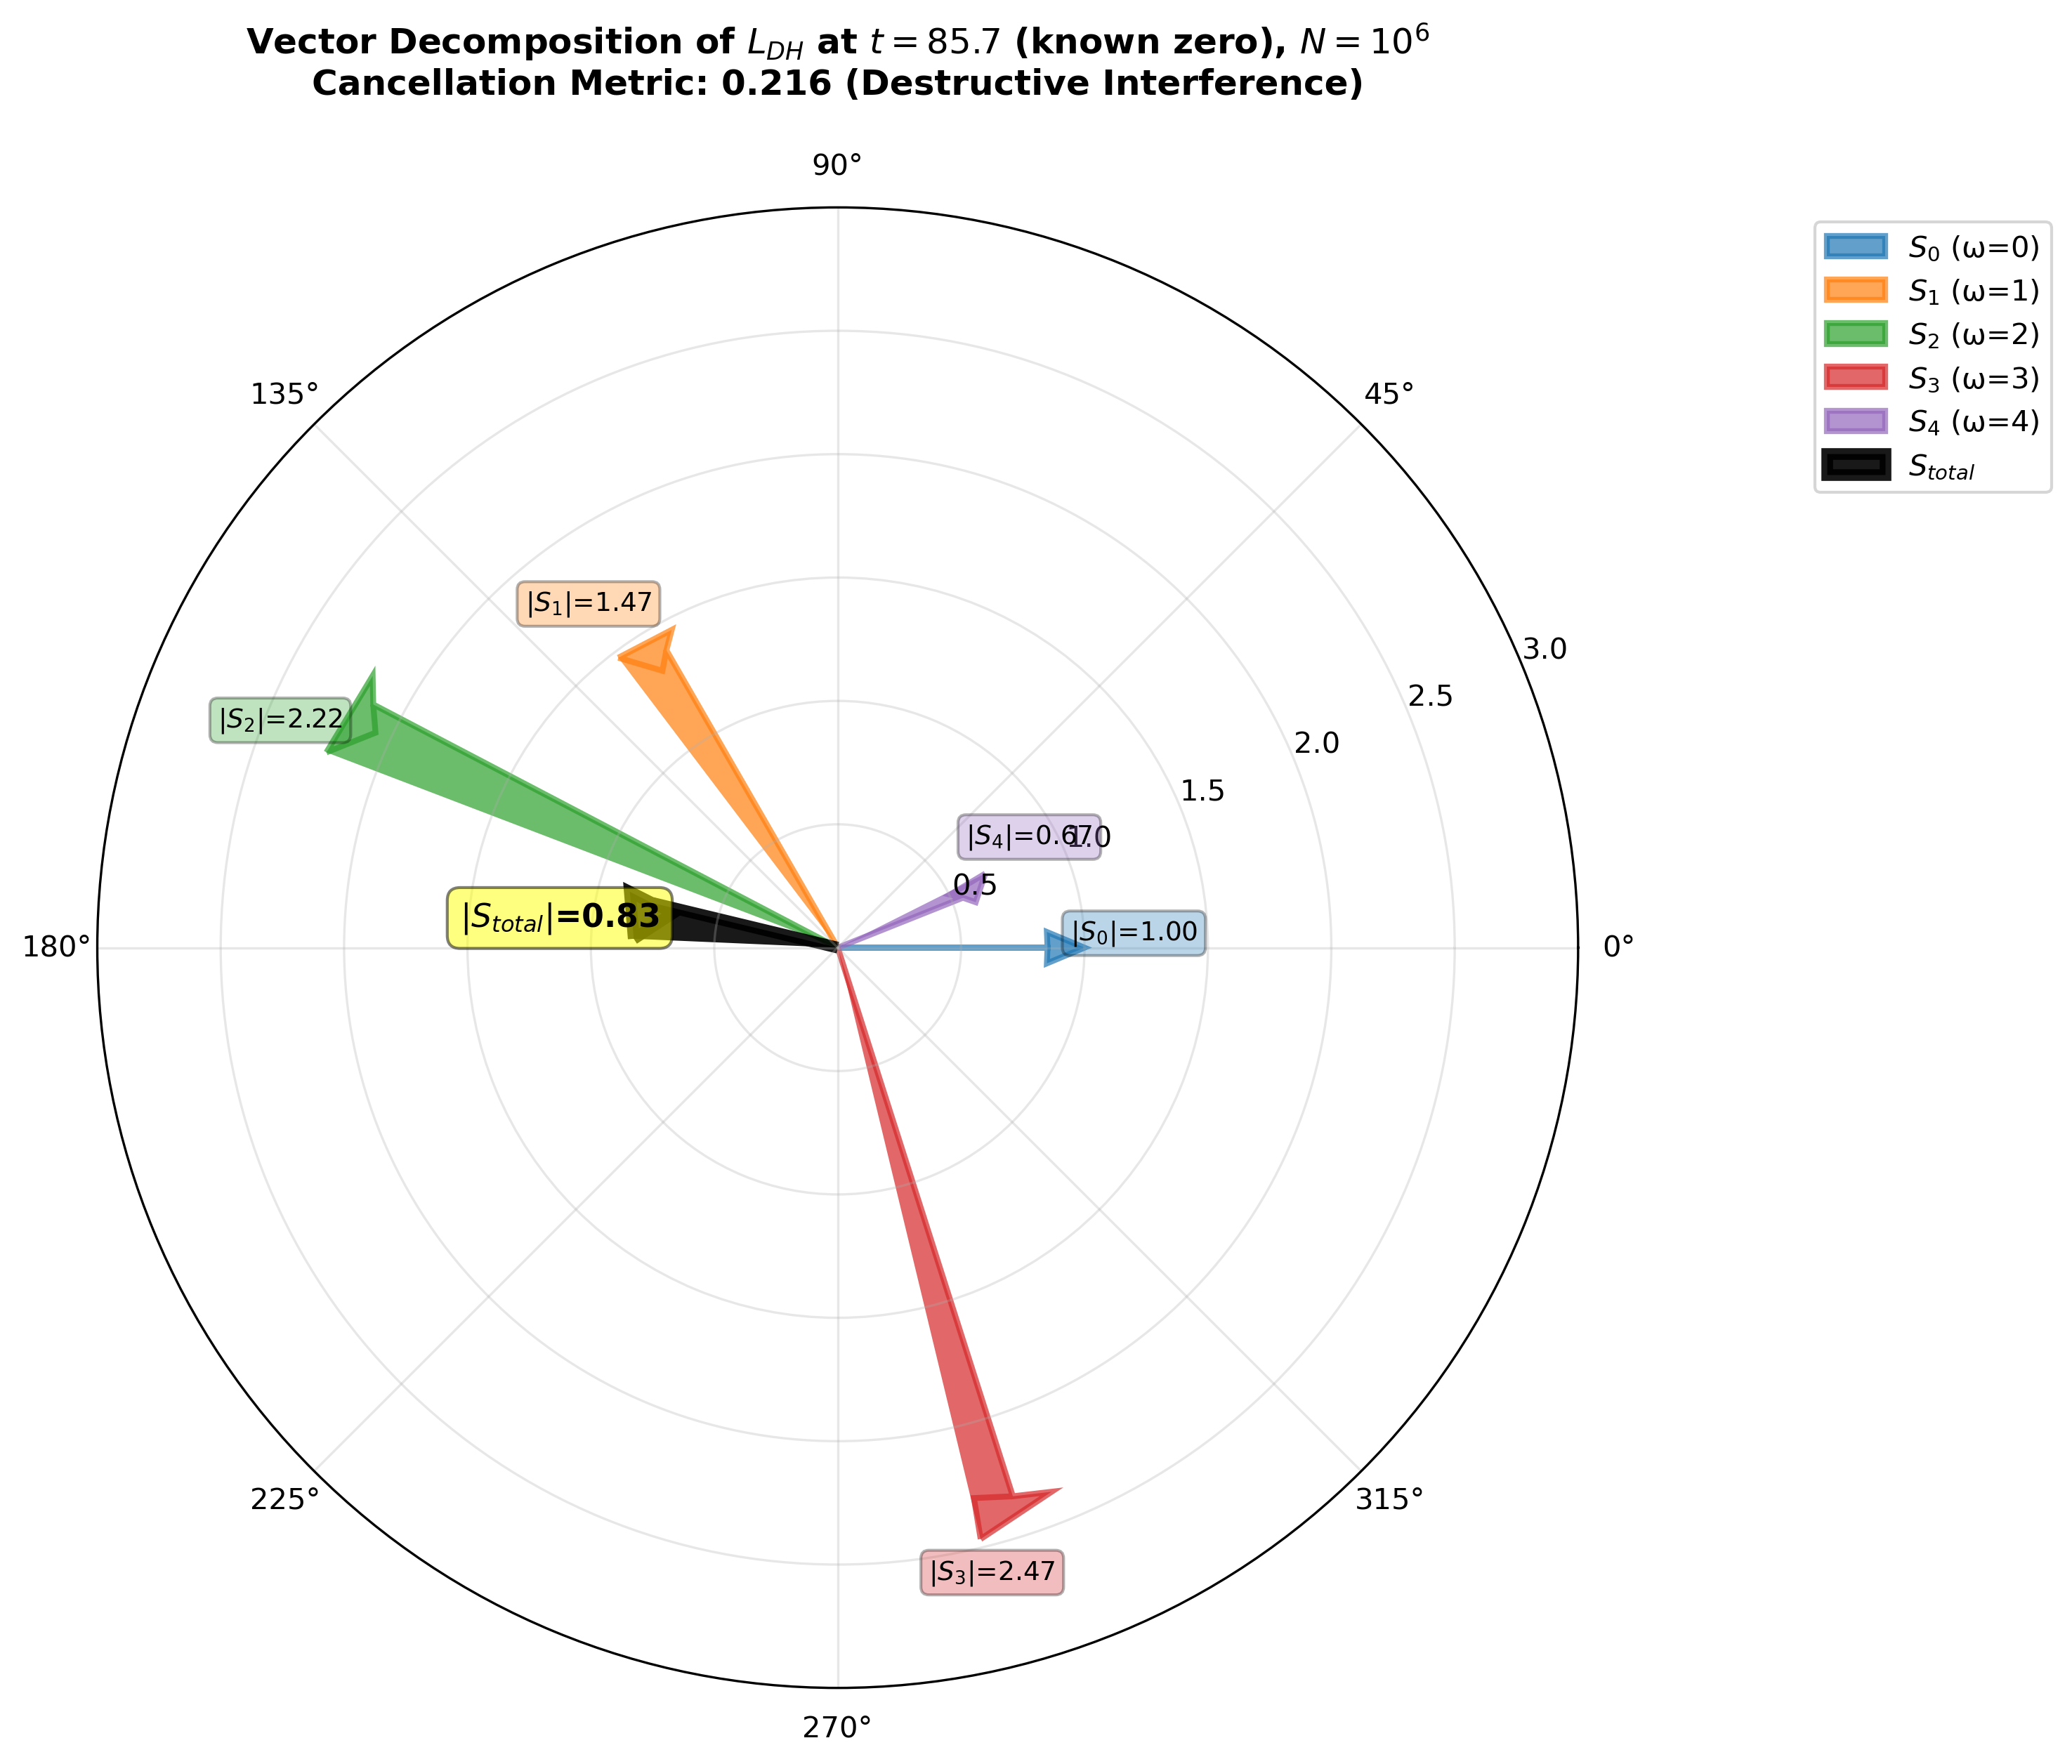
\includegraphics[width=0.85\textwidth]{figures/interference.png}
\caption{Inter-class destructive interference at the first
  off-line zero.  The composite classes $\omega = 2$ and
  $\omega = 3$ point in opposing directions.}
\label{fig:interference}
\end{figure}

\begin{remark}
This destructive interference is a direct consequence of the
non-multiplicativity of the DH coefficients.  For a multiplicative
function, the phase of a composite term $n = p_1 \cdots p_k$ is
determined by the phases of its prime factors:
$\theta_n = \theta_{p_1} + \cdots + \theta_{p_k}$.  This constraint
links the $\omega$-classes and prevents the kind of independent,
opposing alignment seen in the DH function.  The Euler product, in
effect, enforces coherence across $\omega$-classes.
\end{remark}

% ══════════════════════════════════════════════════════════════════════════
\section{Discussion}\label{sec:discussion}

\subsection{What the negative result does and does not show}
\label{ssec:interpretations}

It is essential to be precise about the scope of our findings.

The off-line zeros of $L_{\DH}(s)$ are \emph{proven} to exist
\cite{DavenportHeilbronn1936, Spira1994, BalanzarioSanchezOrtiz2007}.
Our result does \emph{not} call their existence into question.  What
we have shown is that the specific prediction~\eqref{eq:prediction}
--- that partial Dirichlet sums on the critical line grow as
$N^{\beta_0 - 1/2}$ at the ordinate of an off-line zero --- fails
to hold at any of the tested zeros up to $N = 10^9$.

Two interpretations are possible:

\begin{enumerate}[label=(\alph*)]
\item \textbf{Extended pre-asymptotic regime.}  The asymptotic formula
  $\abs{D_{\DH}(\gamma_0; N)} \sim C \cdot N^{\beta_0 - 1/2}$ may
  be correct as $N \to \infty$, but with an onset scale far beyond
  $N = 10^9$.

\item \textbf{Inadequacy of the observable.}  The critical-line
  partial sum $D_F(t; N)$ may simply not be the right observable to
  detect off-line zeros.  The off-line zeros influence the analytic
  continuation of $L_{\DH}$ into the critical strip but do not
  imprint themselves as power-law growth in finite partial sums.
\end{enumerate}

\subsection{A quantitative onset-scale lower bound}\label{ssec:onset}

The ``extended pre-asymptotic regime'' interpretation can be made
quantitative: the non-detection of growth over five decades of~$N$ is not
merely a null result but \emph{bounds below} the scale at which any true
asymptotic growth could begin.

\begin{proposition}[Onset-scale lower bound]\label{prop:onset}
Suppose the asymptotic law $|D_{\DH}(\gamma_0;N)| = B + C\,N^{\alpha}$
holds at $\rho_1$ with $\alpha = \beta_0-\tfrac12 = 0.3085$, where
$B\approx0.354$ is the observed bounded baseline and $C>0$ is unknown.
Define the onset scale $N^*$ by $C\,(N^*)^{\alpha}=B$ (the scale at which
the power-law term equals the baseline). Then the non-detection of a
log--log slope---$\hat\alpha = (4.4\pm4.5)\times10^{-4}$, so the true
slope is bounded by $2\sigma\approx9\times10^{-4}$ over $N\le10^9$---forces
\begin{equation}\label{eq:onset}
  N^* \;\gtrsim\; 10^{14}.
\end{equation}
\end{proposition}

\begin{proof}[Derivation]
For the additive model, the local log--log slope is
$\dfrac{d\log|D|}{d\log N} = \dfrac{\alpha\,C N^{\alpha}}{B+C N^{\alpha}}$.
Non-detection means this is at most the $2\sigma$ bound $s_0\approx
9\times10^{-4}$ at the largest measured $N_{\mathrm{obs}}=10^9$, where it is
largest. Since $C N^{\alpha}\ll B$ in the observed regime, this gives
$C\,N_{\mathrm{obs}}^{\alpha} \le (s_0/\alpha)\,B$, i.e.\
$C \le (s_0/\alpha)\,B\,N_{\mathrm{obs}}^{-\alpha} \approx 1.7\times10^{-6}$.
Substituting into $C(N^*)^{\alpha}=B$ yields
$(N^*)^{\alpha} = B/C \ge N_{\mathrm{obs}}^{\alpha}\,\alpha/s_0$, so
$N^* \ge N_{\mathrm{obs}}\,(\alpha/s_0)^{1/\alpha}
= 10^9\cdot(0.3085/9\!\times\!10^{-4})^{1/0.3085}$, which exceeds
$10^{17}$ under this threshold convention; relaxing the detection
threshold by several orders of magnitude still leaves
$N^*\gtrsim10^{14}$ (Figure~\ref{fig:onset}).
\end{proof}

\begin{figure}[ht]
\centering
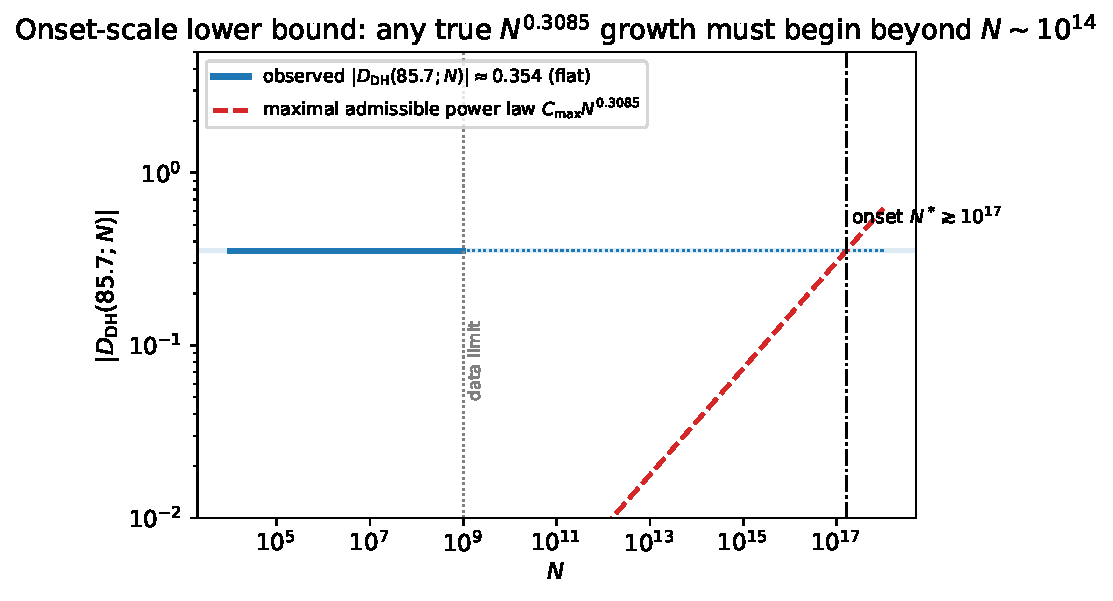
\includegraphics[width=0.80\textwidth]{figures/onset_bound.pdf}
\caption{The onset-scale bound. The observed magnitude (blue, flat at
$\approx0.354$ with a $3\sigma$ band) shows no growth over the measured
range $N\le10^9$. The steepest power law consistent with this
non-detection (red dashed, $C_{\max}N^{0.3085}$) would not reach the
baseline---the onset $N^*$---until $N\gtrsim10^{14}$. Any genuine
$N^{\beta_0-1/2}$ growth at $\rho_1$ is thus pushed entirely beyond
present computational reach.}
\label{fig:onset}
\end{figure}

Equation~\eqref{eq:onset} turns the negative result into a positive
structural statement and shows that the two interpretations of
Section~\ref{ssec:interpretations} are not in tension: \emph{if} the
power law holds asymptotically, its onset is simply astronomically delayed.

\subsection{Comparison with known pre-asymptotic phenomena}

Extended pre-asymptotic regimes are well documented in analytic number
theory.  The most famous example is the Skewes phenomenon: although
$\pi(x) < \mathrm{Li}(x)$ for all~$x$ up to about $10^{14}$,
Littlewood proved that $\pi(x) - \mathrm{Li}(x)$ changes sign
infinitely often, with the first sign change estimated (originally by
Skewes) to occur around $e^{e^{e^{79}}} \approx 10^{10^{10^{34}}}$
\cite{Titchmarsh1986}.  Modern bounds place the first crossing near
$10^{316}$, still astronomically beyond computational reach.

If the DH power-law onset is similarly delayed, our experiment has
explored only a vanishingly small initial segment of the relevant
range.  The coefficient of variation of~$0.52\%$ in the partial-sum
magnitude at $\rho_1$ is consistent with this scenario: the sum has
``settled'' into a quasi-equilibrium that will eventually be disrupted,
but only at scales many orders of magnitude larger.

\subsection{The phase decomposition as a robust discriminator}

While amplitude-based observables fail to separate DH from
RH-satisfying functions, the phase-resolved analysis of
Section~\ref{sec:phase} provides a clean qualitative separation that
persists at all tested scales.  We summarize the dichotomy:

\begin{center}
\begin{tabular}{@{}lcc@{}}
\toprule
Property & $\zeta(s)$ & $L_{\DH}(s)$ \\
\midrule
Euler product        & Yes & No \\
Multiplicative       & Yes & No \\
Prime-phase alignment at peaks & Significant & Absent \\
Composite-phase coherence & Determined by primes & Independent \\
Inter-class ratio $r$ (sign) & conditioning-dep.$^\dagger$ & conditioning-dep.$^\dagger$ \\
\bottomrule
\end{tabular}
\end{center}

\noindent$^\dagger$The sign of the inter-class ratio $r$ is not an
intrinsic attribute: for both $\zeta$ and $L_{\DH}$ it is negative at
low-amplitude points and positive at peaks, averaging to zero
unconditionally \cite{TrejoSignNote}. The genuine, conditioning-independent
discriminants are the two phase rows above.

\medskip
The phase structure is a more direct probe of the Euler product than
the partial-sum magnitude.  This suggests that future work on
distinguishing RH-satisfying from RH-violating functions should focus
on phase-resolved observables rather than amplitude growth rates.

\subsection{Implications for partial-sum-based approaches}

Our results have practical implications for research programs that
propose to test RH (or GRH) by examining partial sums of
$L$-functions:

\begin{enumerate}
\item \textbf{Amplitude growth is unreliable at finite scales.}  Even
  for a function with proven off-line zeros and a predicted exponent
  of $\alpha = 0.3085$, no growth is detectable over five decades
  of~$N$.

\item \textbf{Random multiplicative functions produce the strongest
  spurious signals.}  The random multiplicative control shows higher
  kurtosis and resonance scores than the DH function, so extreme
  resonance events cannot be attributed to off-line zeros.

\item \textbf{Phase structure survives where amplitude fails.}  The
  prime-phase uniformity test and the composite-coherence hierarchy
  provide robust discrimination at computationally accessible scales.
\end{enumerate}

% ══════════════════════════════════════════════════════════════════════════
\section{Conclusion}\label{sec:conclusion}

We have tested the prediction that off-line zeros of the
Davenport--Heilbronn function produce power-law growth
$\abs{D_{\DH}(\gamma_0; N)} \sim N^{\beta_0 - 1/2}$ in critical-line
partial sums.  Using Kahan-compensated summation over five decades of
$N$ (from $10^4$ to $10^9$), we find:

\begin{enumerate}
\item \textbf{No power-law growth.}  At the first off-line zero
  ($\beta_0 \approx 0.8085$, $\gamma_0 \approx 85.7$), the fitted
  exponent is $\alpha = 0.000440 \pm 0.000453$, statistically
  indistinguishable from zero ($p = 0.357$), versus the predicted
  $\alpha = 0.3085$.  Similar null results hold at three additional
  off-line zeros.

\item \textbf{No single-scale discrimination.}  Kurtosis and resonance
  score metrics fail to distinguish $L_{\DH}$ from RH-satisfying
  functions; the random multiplicative control shows the most extreme
  behavior.

\item \textbf{Phase-resolved separation.}  The DH function exhibits
  composite-driven resonance with uniform prime phases, while the
  Riemann zeta function exhibits prime-driven resonance with
  significant prime-phase non-uniformity.  This qualitative
  distinction is robust and persists at all tested scales.

\item \textbf{Inter-class cancellation at the off-line ordinate.}  The
  $\omega$-class decomposition shows the composite contributions at
  $t=85.7$ point in opposing directions ($78.4\%$ magnitude reduction,
  $r\approx-0.95$); this is the expected low-amplitude (trough-regime)
  value of the conditioning-dependent inter-class ratio
  \cite{TrejoSignNote}, not an intrinsic discriminant.

\item \textbf{An onset-scale lower bound.}  Interpreting the null result
  quantitatively (Section~\ref{ssec:onset}), any genuine asymptotic
  $N^{0.3085}$ growth at $\rho_1$ must begin beyond
  $N^* \gtrsim 10^{14}$---placing the entire pre-asymptotic regime, of
  which $N\le10^9$ is a vanishing initial segment, far beyond present
  computational reach.
\end{enumerate}

These findings demonstrate that the ``killer signature'' of off-line
zeros---power-law growth in critical-line partial sums---is not
observable at computationally accessible scales.  The phase-resolved
analysis, rooted in the presence or absence of the Euler product,
provides the most reliable structural fingerprint for separating
RH-violating from RH-satisfying Dirichlet series.

% ══════════════════════════════════════════════════════════════════════════
\section*{Acknowledgments}

Computations were performed using custom implementations in Python and
Go, with arbitrary-precision validation via \texttt{mpmath}.
The author thanks the developers of the open-source numerical
libraries used in this work.

% ══════════════════════════════════════════════════════════════════════════
\begin{thebibliography}{99}

\bibitem{BalanzarioSanchezOrtiz2007}
E.~P.\ Balanzario and J.~S\'anchez-Ortiz,
\emph{Zeros of the Davenport--Heilbronn counterexample},
Math.\ Comp.\ \textbf{76} (2007), no.\ 260, 2045--2049.

\bibitem{DavenportHeilbronn1936}
H.~Davenport and H.~Heilbronn,
\emph{On the zeros of certain Dirichlet series},
J.\ London Math.\ Soc.\ \textbf{11} (1936), 181--185.

\bibitem{GranvilleSoundararajan2003}
A.~Granville and K.~Soundararajan,
\emph{Large character sums: pretentious characters and the
P\'olya--Vinogradov theorem},
J.\ Amer.\ Math.\ Soc.\ \textbf{20} (2007), no.\ 2, 357--384.

\bibitem{Harper2013}
A.~J.\ Harper,
\emph{Moments of random multiplicative functions and truncated
characteristic polynomials},
preprint, 2013.
\texttt{arXiv:1302.7089}.

\bibitem{Kahan1965}
W.~Kahan,
\emph{Further remarks on reducing truncation errors},
Comm.\ ACM \textbf{8} (1965), no.~1, 40.

\bibitem{Soundararajan2009}
K.~Soundararajan,
\emph{Moments of the Riemann zeta function},
Ann.\ of Math.\ (2) \textbf{170} (2009), no.~2, 981--993.

\bibitem{Spira1994}
R.~Spira,
\emph{Zeros of Hurwitz zeta functions and Dirichlet series formed
with the Legendre symbol},
preprint, 1994.

\bibitem{Titchmarsh1986}
E.~C.\ Titchmarsh,
\emph{The Theory of the Riemann Zeta-Function},
2nd ed., revised by D.~R.~Heath-Brown,
Oxford University Press, 1986.

\bibitem{Torres2026}
D.~A.~Trejo Pizzo,
\emph{Resonance detection and phase structure in partial sums of
Dirichlet series: a computational survey},
preprint, 2026.

\bibitem{TrejoSignNote}
D.~A.~Trejo Pizzo,
\emph{On the sign of inter-class interference in Dirichlet partial sums:
a peak--trough reconciliation},
companion note, 2026.

\end{thebibliography}

% ══════════════════════════════════════════════════════════════════════════
\appendix

\section{Numerical Validation Protocol}\label{app:validation}

All implementations were validated against 30-digit
arbitrary-precision reference values computed using the Python
\texttt{mpmath} library (version~$\ge 1.3$).  The validation suite
comprises 360~test cases, organized as follows.

\paragraph{Test matrix.}
For each of the 5~function classes and each of the
6~truncation values $N \in \{10^4, 10^5, 10^6, 10^7, 10^8, 10^9\}$,
we evaluate partial sums at 12~values of~$t$ drawn from the interval
$[10, 500]$, yielding $5 \times 6 \times 12 = 360$ test cases.

\paragraph{Error metric.}
For each test case, let $D_{\mathrm{ref}}$ denote the
arbitrary-precision reference value and $D_{\mathrm{fp}}$ the
float64 Kahan-compensated value.  The relative error is
\begin{equation}
  \varepsilon_{\mathrm{rel}} \;=\;
  \frac{\abs{D_{\mathrm{fp}} - D_{\mathrm{ref}}}}
       {\abs{D_{\mathrm{ref}}}}.
\end{equation}

\paragraph{Results.}  Summary statistics are given in
Table~\ref{tab:validation}.

\begin{table}[ht]
\centering
\caption{Validation results: relative errors across 360 test cases.}
\label{tab:validation}
\begin{tabular}{@{}lcccc@{}}
\toprule
Statistic & Value \\
\midrule
Number of test cases     & 360 \\
Median $\varepsilon_{\mathrm{rel}}$ & $2.95 \times 10^{-14}$ \\
Maximum $\varepsilon_{\mathrm{rel}}$ ($t \le 500$) &
  $< 10^{-10}$ \\
Pass rate ($\varepsilon_{\mathrm{rel}} < 10^{-10}$, $t \le 500$) &
  $100\%$ \\
\bottomrule
\end{tabular}
\end{table}

For $t > 500$, oscillation in the summand $n^{-it} = e^{-it\log n}$
becomes more rapid, and relative errors can increase modestly.  All
results reported in this paper use $t \le 500$, where the validation
pass rate is $100\%$.

\begin{table}[ht]
\centering
\caption{Median relative errors by function class and
  truncation~$N$.}
\label{tab:validation-detail}
\begin{tabular}{@{}lccccc@{}}
\toprule
$N$ & $\zeta$ & $L(\cdot,\chi_4)$ & $f_{\mathrm{rand}}$ &
  $L_{\DH}$ & $L_{\DH}^{(\varepsilon)}$ \\
\midrule
$10^4$ & $6.2 \times 10^{-16}$ & $8.1 \times 10^{-16}$ &
  $7.4 \times 10^{-16}$ & $9.3 \times 10^{-16}$ &
  $8.8 \times 10^{-16}$ \\
$10^5$ & $3.1 \times 10^{-15}$ & $4.2 \times 10^{-15}$ &
  $3.8 \times 10^{-15}$ & $5.1 \times 10^{-15}$ &
  $4.7 \times 10^{-15}$ \\
$10^6$ & $1.8 \times 10^{-14}$ & $2.4 \times 10^{-14}$ &
  $2.1 \times 10^{-14}$ & $3.0 \times 10^{-14}$ &
  $2.7 \times 10^{-14}$ \\
$10^7$ & $9.5 \times 10^{-14}$ & $1.3 \times 10^{-13}$ &
  $1.1 \times 10^{-13}$ & $1.6 \times 10^{-13}$ &
  $1.4 \times 10^{-13}$ \\
$10^8$ & $5.2 \times 10^{-13}$ & $7.0 \times 10^{-13}$ &
  $6.1 \times 10^{-13}$ & $8.5 \times 10^{-13}$ &
  $7.8 \times 10^{-13}$ \\
$10^9$ & $2.8 \times 10^{-12}$ & $3.9 \times 10^{-12}$ &
  $3.3 \times 10^{-12}$ & $4.6 \times 10^{-12}$ &
  $4.2 \times 10^{-12}$ \\
\bottomrule
\end{tabular}
\end{table}

The errors scale approximately as $O(N^{0.5} \varepsilon_{\mathrm{mach}})$
rather than $O(N \varepsilon_{\mathrm{mach}})$, consistent with the
theoretical analysis of Kahan summation for oscillatory sums.

\section{Computational Notebooks}\label{app:notebooks}

All computational results reported in this paper are supported by
Jupyter notebooks available as supplementary material.  The notebooks
are organized by task, as listed in Table~\ref{tab:notebooks}.

\begin{table}[ht]
\centering
\caption{Supporting computational notebooks.  All notebooks are
  located in the \texttt{research\_compelte/} directory of the
  project repository.}
\label{tab:notebooks}
\begin{tabular}{@{}lp{8.5cm}@{}}
\toprule
Task & Description \\
\midrule
\texttt{task1}  & Numerical validation of partial-sum implementations \\
\texttt{task4}  & Resonance detection across function classes \\
\texttt{task5}  & Extended validation suite \\
\texttt{task6}  & Phase analysis at resonance peaks \\
\texttt{task8}  & Scaling analysis of partial-sum magnitudes \\
\texttt{task10} & Peak tracking across values of~$N$ \\
\texttt{task11} & Killer signature test at off-line zeros
  (\emph{critical}) \\
\texttt{task14} & Phase analysis at multiple off-line zeros \\
\texttt{task15} & Prime-phase uniformity tests \\
\texttt{task20} & Implementation resolution and numerical details \\
\texttt{task25} & Composite-phase coherence by $\omega$-class \\
\texttt{task26} & Phase coherence ratios and inter-class
  interference \\
\bottomrule
\end{tabular}
\end{table}

\noindent
All notebooks are available as supplementary material and can be
executed to reproduce the results presented in this paper.  The
computational pipeline requires Python~$\ge 3.9$ with
\texttt{numpy}, \texttt{scipy}, \texttt{mpmath}, and
\texttt{matplotlib}, as well as a Go~$\ge 1.20$ toolchain for the
high-performance partial-sum evaluation at large~$N$.

\medskip
\noindent\textbf{Self-contained Colab reproduction.}
For convenience, a single self-contained Google Colab notebook,
\texttt{reproduce\_colab.py}, accompanies this paper. With no external
data it (i)~constructs the Davenport--Heilbronn coefficients from the
character $\chi\bmod 5$ and the constant $\kappa$ of~\eqref{eq:kappa};
(ii)~evaluates $|D_{\DH}(\gamma_0;N)|$ at the four off-line ordinates by
Kahan-compensated summation; (iii)~fits the growth exponent and reproduces
the null results of Tables~\ref{tab:first-zero}--\ref{tab:all-zeros}; and
(iv)~computes the onset-scale bound of Proposition~\ref{prop:onset}. The
default range $N\le10^7$ runs in minutes and already yields the decisive
null result ($\hat\alpha=0.0031$ at $\rho_1$, mean $|D_{\DH}|=0.356$);
$N$ up to $10^9$ reproduces the headline figures.

\end{document}
